%%%%%%%%%%%%%%%%%%%%%%%%%%%%%%%%%%%%%%%%%%
%%%                                    %%%
%%% (c) Vojtěch Kopal, 2011            %%%
%%%                                    %%%
%%%%%%%%%%%%%%%%%%%%%%%%%%%%%%%%%%%%%%%%%%


\documentclass[12pt,notitlepage]{report}
%\pagestyle{headings}
\pagestyle{plain}

%\frenchspacing % aktivuje použití některých českých typografických pravidel

\usepackage[utf8]{inputenc} % nastavuje použité kódování, uživatelé Windows zamění latin2 za cp1250
\usepackage{a4wide} % nastavuje standardní evropský formát stránek A4
%\usepackage{index} % nutno použít v případě tvorby rejstříku balíčkem makeindex
%\usepackage{fancybox} % umožňuje pokročilé rámečkování :-)
\usepackage{graphicx} % nezbytné pro standardní vkládání obrázků do dokumentu

\usepackage[left=4cm]{geometry} % nastavení dané velikosti okrajů

%\newindex{default}{idx}{ind}{Rejstřík} % zavádí rejstřík v případě použití balíku index

\newtheorem{definition}{Definition}
\newtheorem{example}{Example}

\title{Komunikace a paměť pro plausibilní agenty}   % tyto dvě položky jsou zde v podstatě formálně, ve skutečnosti nejsou nikde 
\author{Vojtěch Kopal} % dále v dokumentu použity

%\date{}

\begin{document}

%\csprimeson % zapne jednoduché psaní českých uvozovek pomocí klasických znaků, ale potom pozor 
             % na originální apostrofy, které budou chybně interpretovány!!!

%%% Následuje první, úvodní, strana bakalářské práce. Jednotlivé položky nahraďte dle vlastních
%%% údajů. Změnit podle konkrétní délky jednotlivých položek můžete i zalomení řádků.
\begin{titlepage}
\begin{center}
\ \\

\vspace{15mm}

\large
Charles University in Prague\\
Faculty of Mathematics and Physics\\

\vspace{5mm}
   
{\Large\bf BACHELOR THESIS}

\vspace{10mm}

%%% Aby vložní loga vše správně fungovalo, je třeba mít soubor logo.eps nahraný v pracovním adresáři,
%%% tj. v adresáři, kde se nachází překládaný zdrojový soubor. Soubor logo.eps je možné získat např.
%%% na adrese: http://www.mff.cuni.cz/fakulta/symboly/logo.eps

\includegraphics[scale=0.3]{logo.eps} 

\vspace{15mm}

%\normalsize
{\Large Vojtěch Kopal}\\ % doplňte vaše jméno
\vspace{5mm}
{\Large\bf Komunikace a paměť pro plausibilní agenty}\\ % doplňte název práce       
\vspace{3mm}
{\Large\bf Communication and memory in plausible agents}\\ % doplňte název práce     
\vspace{5mm}
{\Large Department of Theoretical Computer Science and Mathematical Logic}\\
\end{center}
\vspace{10mm}

\large
\noindent Supervisor: Mgr. Ondřej Sýkora
\vspace{1mm} 

\noindent Study programme: General Computer Science

\vspace{20mm}

\begin{center}
2011
\end{center}

\end{titlepage} % zde končí úvodní strana

\normalsize % nastavení normální velikosti fontu
\setcounter{page}{2} % nastavení číslování stránek
\ \vspace{10mm} 

\noindent Na tomto místě mohou být napsána případná poděkování (vedoucímu práce, konzultantovi, tomu, kdo půjčil software, literaturu, poskytl data apod.). % doplňte vlastní text

\vspace{\fill} % nastavuje dynamické umístění následujícího textu do spodní části stránky
\noindent Prohlašuji, že jsem svou bakalářskou práci napsal(a) samostatně a výhradně s použitím citovaných pramenů. Souhlasím se zapůjčováním práce a jejím zveřejňováním.

\bigskip
\noindent V Praze dne \hspace{\fill}Jméno Příjmení\\ % doplňte patřičné datum, jméno a příjmení

%%%   Výtisk pak na tomto míste nezapomeňte PODEPSAT!
%%%                                         *********

\tableofcontents % vkládá automaticky generovaný obsah dokumentu

\newpage % přechod na novou stránku

%%% Následuje strana s abstrakty. Doplňte vlastní údaje.
\noindent
Název práce: Název bakalářské práce\\
Autor: Jméno autora\\
Katedra (ústav): Název katedry či ústavu\\
Vedoucí bakalářské práce: Jméno se všemi tituly, event. pracoviště\\
e-mail vedoucího: e-mailová adresa vedoucího\\

\noindent Abstrakt:  V předložené práci studujeme ... Uvede se abstrakt v rozsahu 80 až 200 slov. Lorem ipsum dolor sit amet, consectetuer adipiscing elit. Ut sit amet sem. Mauris nec turpis ac sem mollis pretium. Suspendisse neque massa, suscipit id, dictum in, porta at, quam. Nunc suscipit, pede vel elementum pretium, nisl urna sodales velit, sit amet auctor elit quam id tellus. Nullam sollicitudin. Donec hendrerit. Aliquam ac nibh. Vivamus mi. Sed felis. Proin pretium elit in neque. Pellentesque at turpis. Maecenas convallis. Vestibulum id lectus. Fusce dictum augue ut nibh. Etiam non urna nec mi mattis volutpat. Curabitur in tortor at magna nonummy gravida. Mauris turpis quam, volutpat quis, porttitor ut, condimentum sit amet, felis.\\

\noindent Klíčová slova: klíčová slova (3 až 5)

\vspace{10mm}

\noindent
Title: Název bakalářské práce v angličtině\\
Author: Jméno autora\\
Department: Název katedry či ústavu v angličtině\\
Supervisor: Jméno s tituly jako v české verzi, event. pracoviště\\
Supervisor's e-mail address: e-mailová adresa vedoucího\\

\noindent Abstract: In the present work we study ... Uvede se anglický abstrakt v rozsahu 80 až 200 slov. Lorem ipsum dolor sit amet, consectetuer adipiscing elit. Ut sit amet sem. Mauris nec turpis ac sem mollis pretium. Suspendisse neque massa, suscipit id, dictum in, porta at, quam. Nunc suscipit, pede vel elementum pretium, nisl urna sodales velit, sit amet auctor elit quam id tellus. Nullam sollicitudin. Donec hendrerit. Aliquam ac nibh. Vivamus mi. Sed felis. Proin pretium elit in neque. Pellentesque at turpis. Maecenas convallis. Vestibulum id lectus. Fusce dictum augue ut nibh. Etiam non urna nec mi mattis volutpat. Curabitur in tortor at magna nonummy gravida. Mauris turpis quam, volutpat quis, porttitor ut, condimentum sit amet, felis. \\

\noindent Keywords: klíčová slova (3 až 5) v angličtině

\newpage

%%% Následuje text bakalářské práce členěný do kapitol, které se číslují, označí názvy a graficky oddělí.
%%% Nedoporučuje se používat víc než dvě úrovně číslování kapitol, viz příklad níže.

\chapter{Introduction}

In a modern society the amount of information is far behind what one can remember or even process. If we understand that, we realize how important it is to be able to delegate the thinking amongs group. The decision making in groups and teams is a topic covered by several papers. [citation required] Supposing we have limited capacity of memory, we have to distribute the knowledge amongst people around us and communicate with each other so as to gather facts which we currently need to make the decision. 

Our decisions are either consciously or subliminaly based on our needs or drives - former term might be rather connected with human behavior, latter term is used for plausible agents. As in microeconomics we can use an utility as a measure of relative satisfaction \cite{Varian:micro} and see how one manages fulfilling their needs. While attaining the goals we use a knowledge which we store in our memory and which we update regularly. With infinite memory we wouldn’t have any problems to store all information and use it when required; however, we don’t have such memory - our memory is limited. 

What I mean by saying “not to have enough space in our memory” is one is not able to remember everything. Certain pieces of information are fading away as time goes or as one is learning new facts. I want to observer if and how an intensive communication can substitute insufficient memory space with the condition of constant level of utility.

Is it obvious that adding the ability of communication improves the agents'chances to survive in the environment.

I want to observer the relation between amount of communication and used spatial resource-bounded memory. 

This thesis consists of [N] parts. First, I will introduce the topic of agent and possible memory implementations based on concrete examples (Chapter 2). Then I will explain what algorithms, such as growing neural gas, I am going to use in the program (Chapter 3). In \emph{Chapter 4} there is a description of the simulation, agents, their memory and the communication.

\chapter{Related work}

I will use this chapter as an insight into the world of agents and spatial memory. I hope that you will not be disappointed, since there is no 007 in following lines.

\section{Agents}

There are several ways how to explain what or who the agent is. Apart from systems of agents used in philosophy or sociology, we can see a first modern use of agency and agents in economy where economists have substited the human with a simpler agent. They intended to simplify their economic models to be able to actually simulate something. Buyers and sellers are typical examples of agents used in simplified market model in microeconomics (see []). In this context agents are entities in the model which can act based on situation in the model.

For area of artificial intelligence we can use the definition of an agent which can be found in \cite{russel2003ai}. It cannot be more simple:

\begin{definition}{\bf Agent} is just something that acts.
\end{definition} 

Of course it is as general as it could be and for my purposes it is too simple, so I will use another definition which meets better the context of my work.

\begin{definition}{\bf Agent} is something that senses the environment and affects it using its actuators.
\end{definition} 

Having that defined we continue to specific kinds of agent. In this thesis I use several slightly varying terms about agents: {\emph rational, autonomous, plausible and believable}. 

A rational agent refers back to economics where we can find a definition of rational behaviour. Even though it is rather a hypothetical model, as people are usually irrational in their decisions from the economics perspective, their is yet nice definition whereby a rational agent acts as if balancing costs against benefits to arrive at action that maximizes personal advantage (Milton Friedman (1953), Essays in Positive Economics). So simply he does what is or perhaps might be best for him based on his current knowledge of the world.
 
On the other hand, the rational behaviour might be understood in a completely different way. Plausible agents are such agents, where the basic approach is to implement human-like internal processes. One of the well-known example is neural networks, although they are usually used in quite simplified way. Since it is really difficult to implement completely plausible agent, one can see research teams focusing on a specific part of the complex human being. 

Autonomous agents are those agents which are capable of accomplishing useful tasks or are effective problem solvers \cite{Loyall:believableagents}. A

Believable agents are personality-rich autonomous agents with the powerful properties of characters from the arts \cite{Loyall:believableagents}. Now there is just the autonomous agent left. An autonomous agent should be able to accomplish useful task or be an effective problem solver. I would like to add one more term which is going to fit the agents I use. 

Belief-Desire-Intention (BDI) agency model implements the three parts agent's belief, desire and intention and use them when comes to reasoning. A BDI agent is particular part of bounded rational agent who use those three parts to separatly prepare plans which are later executed. What a BDI distinguishes from a simple reactive agent is a reactive agent creates immediate decisions based on current state of environment and inputs of his sensors. On the other hand, a BDI agent uses the three parts:

\begin{itemize}
\item {\bf belief} represents the agent's informational state, for example sensory inputs and information in his memory,
\item {\bf desire} is the agent's motivational state, what he needs to approach, for example he is hungry and he needs to find appropriate food,
\item {\bf intention}, on the other hand, is his immediate decision how he attaing the goal he desires, in other words it is execution of plan, for example next move.
\end{itemize}

\section{Spatial resource-bounded memory}

A memory is something what changes a reactive agent into an agent with ability to learn. It can be used for learing consequances of agent's acts, conditional dependencies in the agent's world (citation for bayesian networks), or spatial information about the environment. The latter one is a kind of memory I used for agents in my simulation. 

A spatial memory is used when agent needs to navigate in usually two or three dimensional space. In short it is a component of an agent which says him where to go when he needs or want to do something. There are several different approaches and a couple of examples are going to be covered in this section. I am going to introduce several existing implementations of spatial memory. Mainly I will focus on if and how they have dealt with bounded resources - either due to implementation restrictions, or when approaching plausibility in their models. 

\subsection{Resource-bounded reasoning}

Rational agents cannot be expected to be able to compute a load of data in a constant time or in a time in which the environment doesn't change much. That is why we have to take into account bounded resources when simulating plausible or rather real agents. What we want to avoid here is the computation of plan takes a long period of time during which the environment changes significantly. As they have mentioned in \cite{Bratman:practicalreasoning}, we could separate plan computation from execting the plan, whereby the plan is prepaired over several executions. In that case we need either to be able to perfectly predict the future, or base our plan on data which does not change at all or is frozen for the given period of time.

\subsection{Short-term and long-term memories}

Generally, when I talk about remembering something I should mention two terms: a long-term memory (LTM) and a short-term memory (STM). Both of which describes a capacity for holding certain amount of information in mind. Apart from the varying amount, the memories differ in availability of such information and a period of time the memories last.       

Short-term memory (...)

Long-term memory (...)

\subsection{Computational memory architectures}

Computational memory architectures for autobiographic agents interacting in complex virtual environment suggested by Ho in \cite{Ho:memoryarchitectures}. works with both short-term and long-term autobigraphic memory, where they have observed agent’s ability to survive comparing to purely reactive agency model. Moreover, they researched whether the narrative communication amongst agents somehow positively influence those agents. They have separately experimented with three types of agents: purely reactive (PR), short-term memory (STM) and long-term memory (LTM). Purely reactive agent walks randomly around the environment avoiding obstacles and searching for resource objects to fulfill his needs. What a pure reactivity means is the agent moves randomly until an event occurred such as a collision with obstacle or a resource object detection.

STM agents in \cite{Ho:memoryarchitectures} further extend the model of purely reactive agents and add a Track-back memory system in addition to the reactive behaviour. Each time an agent deals with an event (e.g. collision, or resource object) he puts such information into his memory. They refer to this as an event-based memory entry making mode. Those events are kept in a linear list of a finite size, whereby the oldest events are cut off. The memory is used when an internal variable is over threshold. That is the moment when agent searches in his memory for an information about relevant resource object. If he succeeded, he retrospectively undoes all memorized states leading to the relevant one. So, what they actually store in memory is an agent’s current state: where he was and what he perceived. While attaining imperfection in retrieving information from short-term memory, they introduced noise distortion using Gaussians.

Long-term memory model is mostly based on psychological autobiographic memory models. There are three parts that are involved in the reasoning process: Event specific knowledge (ESK), Event reconstruction process (ER) and Event filtering and ranking process.

\subsection{Inspirations for my work}



%Former one is responsible for storing event history in a similar way as the event-based memory entry making mode. A stored record contains what objects and environment were around the agent, and values of internal variables. Those values are used as various kinds of keys: match key, search key, and conditions, where search key means the resource which can be obtained if conditions hold in the area specified by match key. 

%As in PR model, the ER is fired when there is an internal variable which is below the threshold. At that moment, the agent goes through ESK and search for relevant record. Such a record has to have an equivalent search key to the type of the low internal variable. It is possible for ER to return more than one relevant record. A reconstruction of appropriate number of events leading to the state described by the record is one important part of the following EFR processes. To reach the desired state we can either Redo the memorized steps which had led to the state, or we can Undo the steps which followed, that means to go through them in a reverse order. 

%Finally, I have mentioned that ER can resolve more than one record, which happens after longer period of time when an agent luckily survived in the environment and, subsequently, managed to fill his ESK with sufficient amount of information. At that moment, there has to be a filtering process, which chooses the best record to be proceeded. EFR processes first filter out records that do not match current state of the environment and then order the rest according to how much they better off the agent’s internal variables.

%As an addition to LTM agents they introduced communicative agents with long-term memory, which are able to share their knowledge among each other. First, they extended the structure of ESK, so as to keep a variable about who is the source of the records. Then they defined a communication protocol between two agents, whereby one agent has a role of story-teller and the other one is a listener. The listener ask the story-teller about a object resource and story-teller returns a best story generated by the same process he normally during his reasoning process.

%During experiments they measured the lifespan of agents, and also observed levels of internal variables for sample agents representing one of each suggested models. It was expected that more complex memory structures led to better results and such assumptions were proved correct. A combination of RTM and LTM was clearly the best model and agents with this model where able to live with the least drops in their internal variables and generally their lives were rather stable comparing to others.

%[“What is interesting in it for me”]

%The suggested RTM and LTM models of agents are more than interesting to be implemented in my simulation. There has to be a couple of minor changes, though, as I am working with a simpler environment comparing to the one used in the work described above. The changes will influence the structure of memory records in both RTM and LTM. Also the communication protocol will be different and I am going to introduce it later in this thesis.



\chapter{Used methods and algorithms}

In previous chapter I have introduced you to several kinds of agents, how they can be used and also what a spatial memory is. I have briefly prepaired you for the next chapters, where I will explain my contribution to this area. This chapter is going to cover the used algorithms and computational methods I have studied and implemented in my work. 

The first subsection disserts on the implementations of agents' memory and in detail describes fundamental parts. Both the Growing Neural Gas and the Quad..blah are used as memory storages to handle spatial information about the environment with bounded resources.

\section{Growing Neural Gas}   
\label{usedalgo:gng}

\subsection{Topology learning}

Processing an enormous spatial data about an environment is computationaly demanding when for example we want to navigate in that environment. A topology learning or recognition can help us to create a representation such as topological map which can be viewed as a graph and which makes reasoning in that environment much easier. Rather complex understanding of topology in an indoor space using Bayesian programming has been shown in \cite{Tapus:topologylearning}. It goes much farther than I need to. 

Based on competitive Hebbian learning (CHL) method \cite{Martinetz:chl} and Neural Gas (NG) \cite{Martinetz:ng} Bern Fritzke suggested earlier mentioned Growing Neural Gas \cite{Fritzke:gng}, an unsupervised learning method for finding a topological structure which reflects the topology of the data distribution. Although the combination of both CHL and NG is an effective method for topology learning, there are some flaws in practical application as it requires an initial setup of number of nodes/centers that are used. This fact prevents the method from adequately describing the topology, when a different number of nodes would work better.

As Fritzke described the algorithm uses a set of nodes and edges that connects the nodes. A simplified describtion of algorithm from \cite{Fritzke:gng} in context of two-dimensional space follows:

\begin{enumerate}
\item Add two nodes at random position onto canvas
\item Generate input signal based on the data distribution (its probability density)
\item Find the nearest node $n_1$ and second nearest node $n_2$ to the signal
\item Increment the age of all edges leading from node $n_2$
\item Add the squared distance between the input signal and the nearest unit in
input space to a local counter variable $\Delta error(n_{1})$
\item Moved node $n_1$ and its topological neighbors towards the signal (according to parametres $epsilon_{winner}$ and $epsilon_{neighbour}$)
\item Remove all edges with an age larger than $a_{max}$
\item Generate new nodes (see \cite{Fritzke:gng}) using variable $alpha$
\item Decrease all error variables by multiplying them with a constant $beta$
\item Go to 1.
\end{enumerate}

For the purpose of this work I want to use this algorithm to learn a topology of data which dynamically changes through the time. We have to setup the variables for this agorithm $alpha$, $beta$, $epsilon_{winner}$, $epsilon_{neighbour}$ and maximal number of nodes. In following subsection I am going to introduce you to the experimenting with this algorithm.

\subsection{Experiments on dynamic data}

As I have mentioned previously I had to setup the variables so as to be able to use Growing Neural Gas method properly. To attain this goal I have made a Java programm which tests various combinations of variables' values and finds the best one. It has sequently run the algorithm for a given number of steps and measured the \emph{score} (see \ref{usedalgo:scoremethod}).

\begin{figure}
\begin{lstlisting}[language=Pascal]
procedure Score()
  (px, py, pvar) <- GetProbableGauss()
  (rx, ry, rvar) <- GetRealGauss()
  
  sqDistance <- (px - rx)*(px - rx) + (py - ry)*(py - ry)
  sqSize <- (pvar + rvar)*(pvar + rvar)
  
  score <- sqDistance / sqSize
  
  return score
end
\end{lstlisting}       
\caption{The \emph{SCORE} method}
\label{usedalgo:scoremethod}
\end{figure}
       
\begin{figure}      
\begin{center}
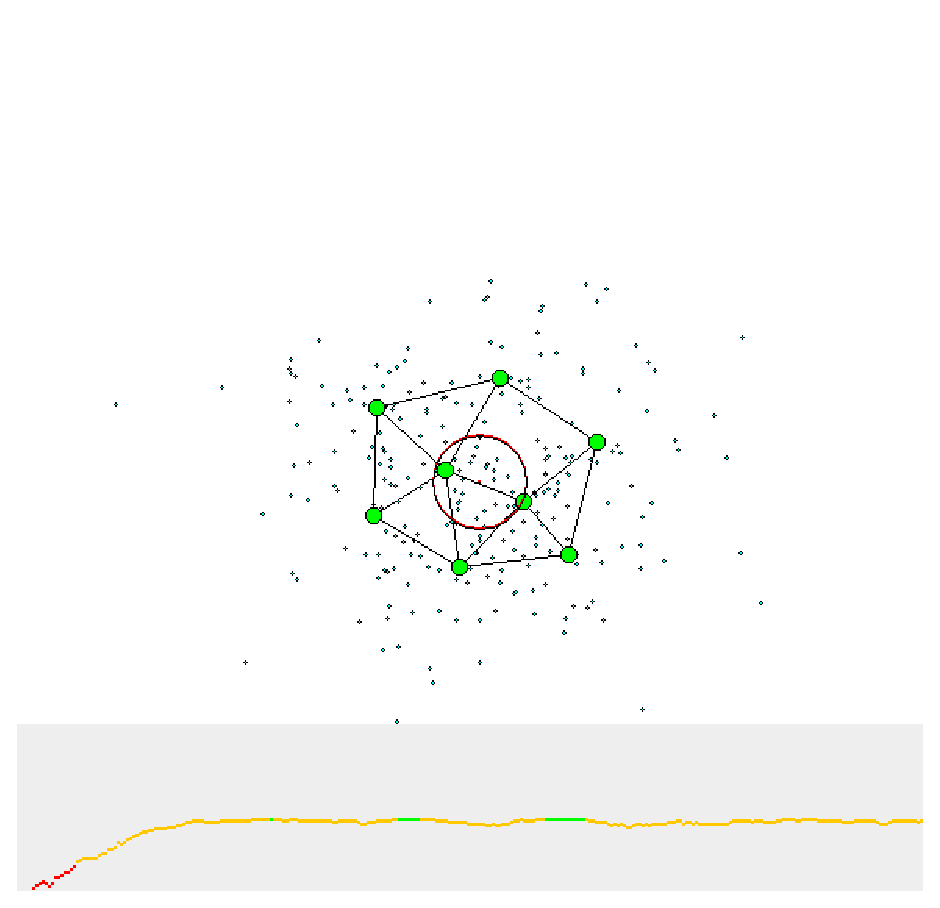
\includegraphics[scale=0.75]{images/gng/experimental_setup.eps}    
\caption{Screenshot showing the process of searching optimal variable values. The visualization has been made for testing purposes in the first place, but it nicely shows what had been lately paralelly computed. The bottom part of the picture shows the SCORE value throughout the simulation. {\emph (Red color means $SCORE > 0.05$, orange is $SCORE > 0.001$ and green is $SCORE <= 0.001$)} }
\end{center}                          
\label{usedalgo:gngexperimentscreen}
\end{figure}

\begin{figure}          
\begin{itemize}
\item $alpha \in \{0.0, 0.2, 0.4, 0.5, 0.6, 0.8, 1.0\}$
\item $beta \in \{0.0, 0.00001, 0.00005, 0.0001, 0.001, 0.005, 0.01, 0.5, 0.1, 0.5, 1.0\}$
\item $epsilon_{winner} \in \{0.0, 0.001, 0.005, 0.01, 0.1, 0.2, 0.5, 1.0\}$
\item $epsilon_{neighbour} \in \{0.0, 0.0001, 0.0006, 0.001, 0.005, 0.05, 0.1, 0.2\}$
\item $maxNodes \in \{4, 8, 16, 32\}$
\end{itemize}
\caption{Domains of variables for the experimental learning of best values.}
\label{usedalgo:gngexperimentdomains}
\end{figure}

A total number of possible combinations is equal to 19712. For each such a combination I have run 10000 steps of GNG learning sequence and measured the average score. Each sequence took aproximately 108 seconds and all the experiment was computed paralelly using 30 threads.

The best results which were avarage $SCORE < 10^{-11}$ is shown in a table \ref{usedalgo:gngexperimentresults}.

\begin{table}
\begin{center}
\begin{tabular}{ccccc|c}

$alpha$ & $beta$ & $epsilon_{winner}$ & $epsilon_{neighbour}$ & $numNodes$ & $SCORE$ \\
\hline
0.0 & 1.0 & 0.0050 & 0.0 & 16 & $3.8*10^{-12}$ \\
0.5 & 0.0 & 0.01 & 1.0E-4 & 8 & $5.1*10^{-12}$ \\   
0.5 & 0.0010 & 0.1 & 0.0010 & 8 & $8.8*10^{-12}$ \\ 
0.5 & 1.0 & 0.0 & 1.0E-4 & 8 & $3.1*10^{-12}$ \\     
0.8 & 1.0E-5 & 0.0010 & 1.0E-4 & 32 & $7.4*10^{-12}$ \\
0.8 & 1.0E-5 & 0.0050 & 6.0E-4 & 8 & $4.3*10^{-12}$ \\

\end{tabular}      
\caption{\label{usedalgo:gngexperimentresults}Variable values with best average SCOREs}
\end{center}
\end{table}

\section{Grid}
\label{sec:grid}

The idea for this data structure representing resource-bounded memory is based on \cite{Brom:placeandobjects}. What differs in my work from their observed environment is agents in my simulation act in a homogeneous space which cannot be differentiated in a way the mentioned simulation does. To solve this issue I have simply differentiated the environment into grid 4x4, where each cell works as the place in \cite{Brom:placeandobjects}. 

Each cell is given two variables {\emph positive} and {\emph negative} both of which are set to zero and increased throughout the simulation. When an agent sees at least half of that area determined by the cell, if he sees any food, he increase the {\emph positive} variable. If the agent search for food and he cannot see any, he increase the {\emph negative} variable.

When the grid is later asked whether there is food at specific cell, it answers according to this method with parametr $\alpha$ to be found:

\begin{equation} ANSWER = \alpha\times positive - negative 
\end{equation}
 
Similary I will use this structure to keep spatial information about the environment in the simulation.


%%% Seznam literatury
%%%
%%% Literatura se řadí abecedně. Úvádí se pouze literatura, na kterou se v textu odkazuje.
%%% Při odkazu na knihu se vždy uvádějí čísla stránek.

\addcontentsline{toc}{chapter}{Bibliography}
\bibliographystyle{plain}
\bibliography{bc_thesis}
  
\end{document}
